\documentclass[11pt]{article}
\usepackage{graphicx}
\usepackage{amsmath, amssymb, float}
\usepackage{mathtools}
\usepackage{enumitem}
\allowdisplaybreaks

\DeclareMathOperator{\EX}{\mathbb{E}}% expected value
\DeclareMathOperator{\Var}{\operatorname{Var}}% variance
\DeclareMathOperator{\Span}{\operatorname{span}}% span
\DeclareMathOperator{\Ad}{\operatorname{Ad}}% Adjoint
\newcommand{\pd}[2]{\frac{\partial #1}{\partial #2}} % partial derivatives

\title{ROB 530 Project Notes}
\author{rlybrdgs }

\begin{document}

\maketitle

\begin{figure}[H]
    \centering
    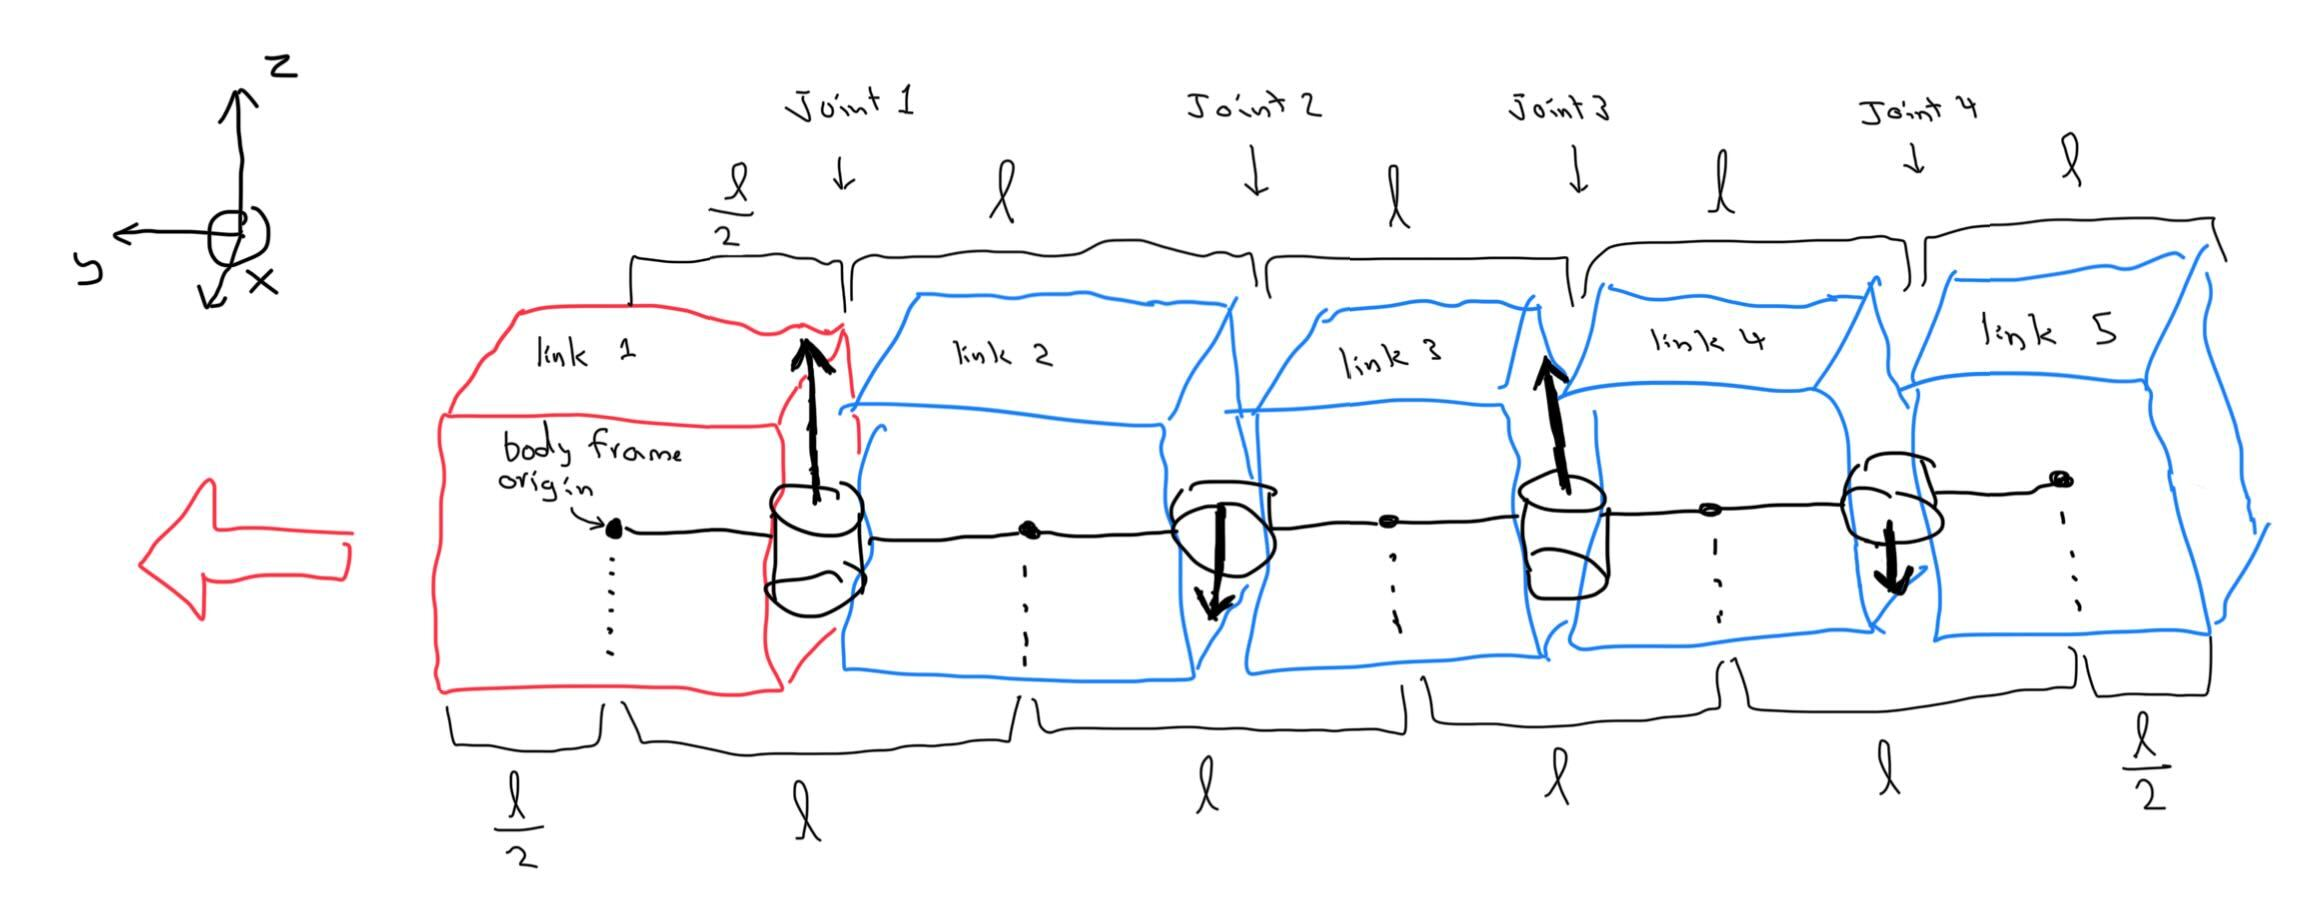
\includegraphics[width=1.2\textwidth]{snake_diagram.jpg}
    \caption{Example diagram of 4 joint snake robot.}
\end{figure}
\newpage 

\section{Forward Kinematics}
\begin{align*}
    g_{st}(\theta) &= e^{\hat{\xi}_1 \theta_1} e^{\hat{\xi}_2 \theta_2} \cdots e^{\hat{\xi}_N \theta_N} g_{st}(0) \\
    g_{si}(\theta) &= e^{\hat{\xi}_1 \theta_1} e^{\hat{\xi}_2 \theta_2} \cdots e^{\hat{\xi}_{i-1} \theta_{i-1}} g_{si}(0) \\
    \xi_i &= \begin{bmatrix}
        -\omega_i \times q_i \\
        \omega_i
    \end{bmatrix} \\
    \omega_i &= \begin{cases}
        \begin{bmatrix}
            1 & 0 & 0
        \end{bmatrix}^\top & i \text{ is even} \\
        \begin{bmatrix}
            0 & 0 & 1
        \end{bmatrix}^\top & i \text{ is odd}
    \end{cases} \\
    q_i &= \begin{bmatrix}
        0 \\ \frac{l}{2} + \sum_{j=1}^{i-1} l \\ 0
    \end{bmatrix} = \begin{bmatrix}
        0 \\ l(i - \frac{1}{2}) \\ 0
    \end{bmatrix} \\
    \xi_i &= \begin{cases}
        \begin{bmatrix}
            0 & 0 & -l(i-\frac{1}{2}) & 1 & 0 & 0
        \end{bmatrix}^\top & i \text{ is even} \\
        \begin{bmatrix}
            l(i-\frac{1}{2}) & 0 & 0 & 0 & 0 & 1
        \end{bmatrix}^\top & i \text{ is odd}
    \end{cases} \\
    g_{si}(0) &= \begin{bmatrix}
        1 & 0 & 0 & 0 \\
        0 & 1 & 0 & l(i-1) \\
        0 & 0 & 1 & 0 \\
        0 & 0 & 0 & 1
    \end{bmatrix}
\end{align*}

\section{Prediction Step}
\begin{align*}
    \mathbf{x}_k &= \begin{bmatrix}
        a_k \\ q_k \\ \omega_k %\\ \theta_k \\ \dot{\theta}_k
    \end{bmatrix} \in \mathbb{R}^{10} \\
    \mathbf{x}_k &= f(\mathbf{x}_{k-1}, \mathbf{u}_k) + \mathbf{w}_k \\
    &= \begin{bmatrix}
        e^{-\tau \Delta t} a_{k-1} \\
        \exp\left(-\frac{1}{2} \Psi(\omega_{k-1}) \Delta t\right) q_{k-1} \\
        \omega_{k-1} \\
        % \theta_{k-1} + \dot{\theta}_{k-1} \Delta t \\
        % (1 - \lambda) \dot{\theta}_{k-1} + \lambda \mathbf{u}_k
    \end{bmatrix} \\
    q_k &= \exp\left(-\frac{1}{2} \Psi(\omega_{k-1}) \Delta t\right) q_{k-1} \\
    &= \left(I \cos\left(\frac{\|\omega_{k-1} \Delta t\|}{2}\right) - \frac{1}{2} \begin{bmatrix}
        0 & -\omega^x \Delta t & \omega^y \Delta t & \omega^z \Delta t \\
        -\omega^x \Delta t & 0 & -\omega^z \Delta t & -\omega^y \Delta t \\
        -\omega^y \Delta t & \omega^z \Delta t & 0 & -\omega^x \Delta t \\
        -\omega^z \Delta t & -\omega^y \Delta t & \omega^x \Delta t & 0
    \end{bmatrix} \frac{\sin\left(\|\omega_{k-1} \Delta t\|\right)}{\|\omega_{k-1} \Delta t\|}\right) q_{k-1} \\
    % F_k &= \pd{f}{\mathbf{x}_{k-1}} = \begin{bmatrix}
    %     e^{-\tau \Delta t} & 0 & 0 & 0 & 0 \\
    %     0 & \pd{q_k}{q_{k-1}} & \pd{q_k}{\omega_{k-1}} & 0 & 0 \\
    %     0 & 0 & 1 & 0 & 0 \\
    %     0 & 0 & 0 & 1 & \Delta t \\
    %     0 & 0 & 0 & 0 & 1
    % \end{bmatrix} \\
    F_k &= \pd{f}{\mathbf{x}_{k-1}} = \begin{bmatrix}
        Ie^{-\tau \Delta t} & 0 & 0 \\
        0 & \pd{q_k}{q_{k-1}} & \pd{q_k}{\omega_{k-1}} \\
        0 & 0 & I \\
    \end{bmatrix} \\
    \pd{q_k}{q_{k-1}} &= TODO \\
    \pd{q_k}{\omega_{k-1}} &= TODO \\
\end{align*}

\section{Update Step}
Variable Conventions:
\begin{itemize}
    \item $q_k$ or $R_k$ is rotation from VC frame to world frame at time $k$
    \item $a_k$ is acceleration of VC frame in world frame, expressed in the world frame at time $k$
    \item $\omega_k$ is angular velocity of VC frame in world frame, expressed in the VC frame at time $k$
    \item $g_{si}(\theta)$ is transform from link $i$ to snake head frame, given joint angles $\theta$
    \item $C_k$ is rotation from VC frame to snake head frame at time $k$
    \item $W_k^i$ is rotation from link $i$ to VC frame at time $k$
    \item $\alpha_k$ is the measured acceleration of link $i$ in the world frame, expressed in the link frame at time $k$
    \item $\gamma_k$ is the measured angular velocity of link $i$ in the world frame, expressed in the link frame at time $k$
\end{itemize} 
\begin{align*}
    g_{si}(\theta_k) &= \begin{bmatrix}
        R_k^i & p_k^i \\
        0 & 1
    \end{bmatrix} \\
    W_k^i &= C_k^\top R_k^i \\
    \mathbf{z}_k &= \begin{bmatrix}
        \alpha_k \\ \gamma_k
    \end{bmatrix} \in \mathbb{R}^{6N} \\
    \hat{\alpha}_k^i &= (W_k^i)^\top R_k^\top (g + a_k) + \hat{a}^i_{\text{internal}} \\
    % &= (C_k^\top R_k^i)^\top R_k^\top (g + a_k) + \hat{a}^i_{\text{internal}} \\
    &= (C_k^\top R_k^i)^\top R_k^\top (g + a_k) + C_k^\top \ddot{p}_k^i \\
    \hat{\gamma}_k^i &= (W_k^i)^\top \omega_k + \hat{\omega}^i_{\text{internal}} \\
    \hat{\omega}^i_{\text{internal}} &= C_k^\top\left(\dot{R}_k^i(R_k^i)^\top\right)^\vee \\
    &= \left(\dot{W}^i_k(W_k^i)^\top\right)^\vee \approx \frac{\text{Log}\left(W_k^i(W_{k-1}^i)^\top\right)}{\Delta t} \approx \left(\frac{W_k^i(W_{k-1}^i)^\top}{\Delta t} - I\right)^\vee
\end{align*}
\begin{align*}
    \hat{\mathbf{z}}_k &= h(\mathbf{x}_k) \\
    &= \begin{bmatrix}
        % \theta_k \\
        (W_k^1)^\top R_k^\top (g + a_k) + \hat{a}^1_{\text{internal}} \\
        \vdots \\
        (W_k^N)^\top R_k^\top (g + a_k) + \hat{a}^N_{\text{internal}} \\
        (W_k^1)^\top \omega_k + \hat{\omega}^1_{\text{internal}} \\
        \vdots \\
        (W_k^N)^\top \omega_k + \hat{\omega}^N_{\text{internal}} \\
    \end{bmatrix} \\
    % \hat{a}^i_{\text{internal}} &= C_k^\top \ddot{p}_k^i \\
    H_k &= \pd{h}{\mathbf{x}_k} = \begin{bmatrix}
        \pd{\hat{\alpha}^1_k}{a_k} & \pd{\hat{\alpha}^1_k}{q_k} & \pd{\hat{\alpha}^1_k}{\omega_k} \\
        \vdots & \vdots & \vdots \\
        \pd{\hat{\alpha}^N_k}{a_k} & \pd{\hat{\alpha}^N_k}{q_k} & \pd{\hat{\alpha}^N_k}{\omega_k} \\
        \pd{\hat{\gamma}^1_k}{a_k} & \pd{\hat{\gamma}^1_k}{q_k} & \pd{\hat{\gamma}^1_k}{\omega_k} \\
        \vdots & \vdots & \vdots \\
        \pd{\hat{\gamma}^N_k}{a_k} & \pd{\hat{\gamma}^N_k}{q_k} & \pd{\hat{\gamma}^N_k}{\omega_k} \\
    \end{bmatrix} = \begin{bmatrix}
        \pd{\hat{\alpha}^1_k}{a_k} & \pd{\hat{\alpha}^1_k}{q_k} & 0 \\
        \vdots & \vdots & \vdots \\
        \pd{\hat{\alpha}^N_k}{a_k} & \pd{\hat{\alpha}^N_k}{q_k} & 0 \\
        0 & 0 & \pd{\hat{\gamma}^1_k}{\omega_k} \\
        \vdots & \vdots & \vdots \\
        0 & 0 & \pd{\hat{\gamma}^N_k}{\omega_k} \\
    \end{bmatrix} \\
    \pd{\hat{\alpha}^i_k}{a_k} &= \pd{}{a_k} \left((W_k^i)^\top R_k^\top (g + a_k)\right) + \pd{}{a_k} \hat{a}^i_{\text{internal}} \\
    &= \pd{}{a_k} \left((W_k^i)^\top R_k^\top g\right) + \pd{}{a_k} \left((W_k^i)^\top R_k^\top a_k\right) + 0 \\ 
    &= 0 + \pd{}{a_k} \left((W_k^i)^\top R_k^\top a_k\right) \\
    &= (W_k^i)^\top R_k^\top \\
    \pd{\hat{\alpha}^i_k}{q} &= \begin{bmatrix}
        \pd{\hat{\alpha}^i_k}{q_x} & \pd{\hat{\alpha}^i_k}{q_y} & \pd{\hat{\alpha}^i_k}{q_z} & \pd{\hat{\alpha}^i_k}{q_w}
    \end{bmatrix} \\
    \pd{\hat{\alpha}^i_k}{q_j} &= \pd{}{q_j} \left((W_k^i)^\top R_k^\top (g + a_k)\right) + \pd{}{q_j} \hat{a}^i_{\text{internal}} \\
    &= (W_k^i)^\top \pd{}{q_j} \left( R_k^\top (g + a_k)\right) + 0 \\
    &= (W_k^i)^\top \pd{R_k^\top}{q_j} (g + a_k) = (W_k^i)^\top \left(\pd{R_k}{q_j}\right)^\top (g + a_k) \\
    \pd{\hat{\gamma}^i_k}{\omega_k} &= \pd{}{\omega_k} \left((W_k^i)^\top \omega_k\right) + \pd{}{\omega_k} \hat{\omega}^i_{\text{internal}} \\
    &= (W_k^i)^\top \\
\end{align*}

\end{document}